
\section{Data distribution system}
The collision and simulated data are stored at different tiers located at 
different places in the world. Being a very large collaboration, where thousands
of people from across the world work on the same data, the CMS distributes 
its data in such a way that any user can access these through the worldwide
LHC grid. The data distribution system is divided into various tiers such as 
tier-0 (T0), tier-1 (T1), and tier-2 (T2) depending on the type of operations
performed on the data. These are located at different places, as shown in 
Figure~\ref{fig:data_tier}. A brief description of all the data tiers is 
given below.
\begin{figure}
  \begin{center}
  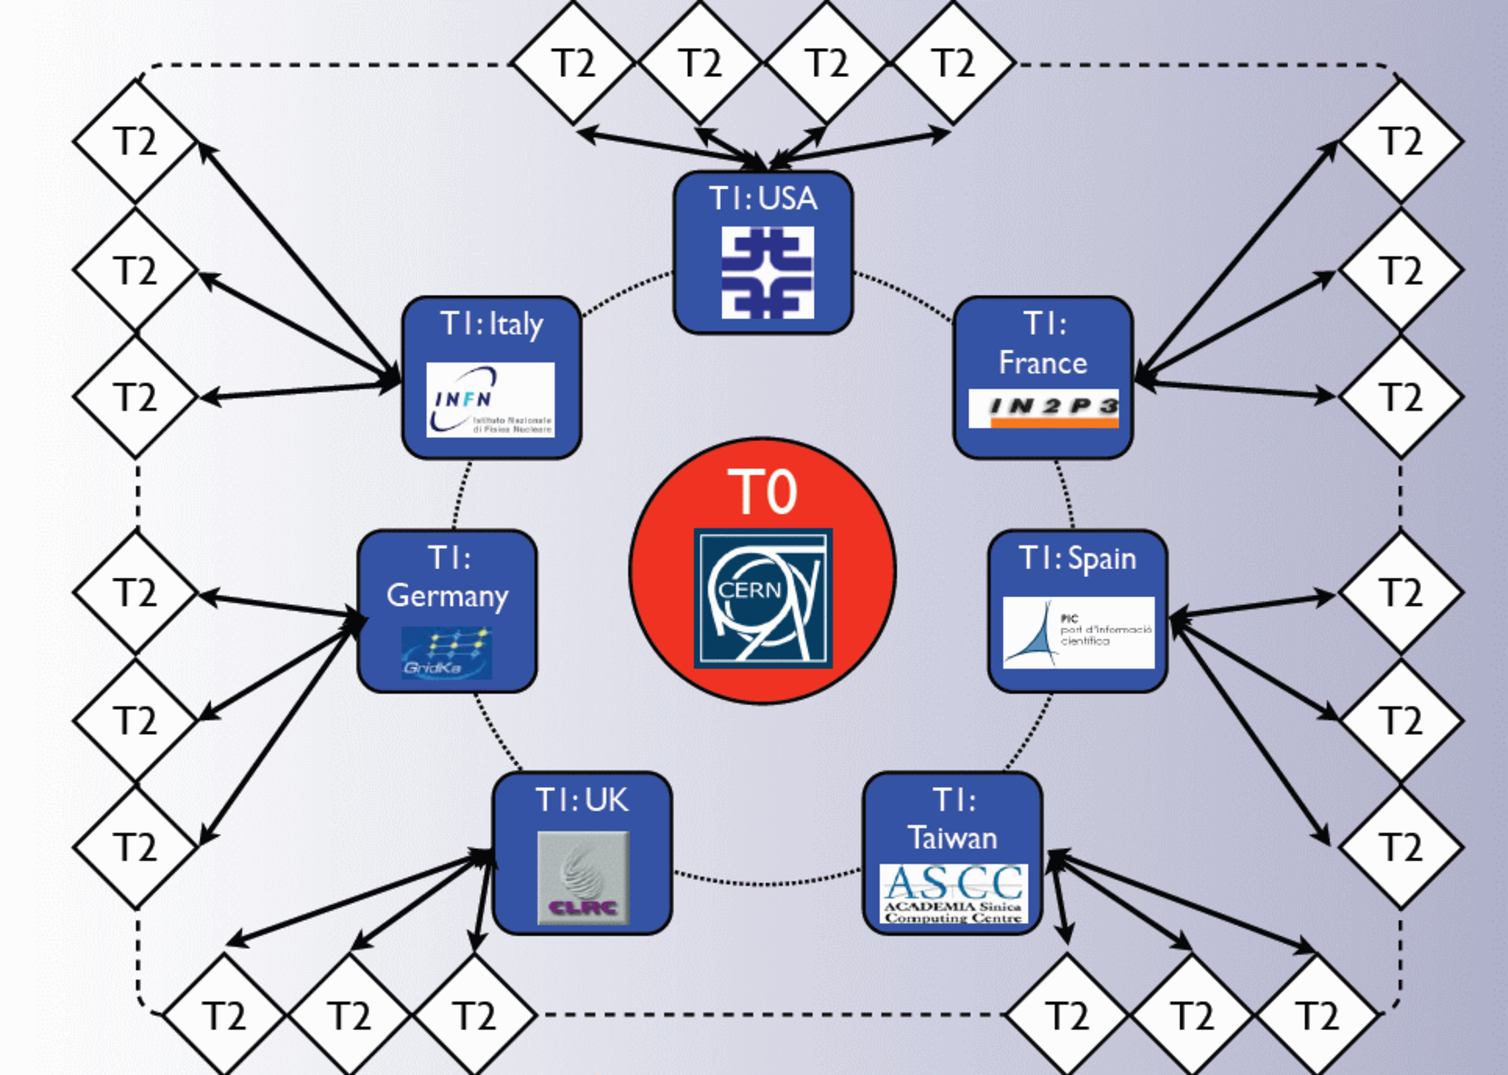
\includegraphics[width=0.70\linewidth]{Experiment/CMS/Image/data_tier.pdf}
	  \caption{Location of different data acquisition systems \cite{triDAS}.
	  The T0 is located at CERN, T1s are located in 7 different places,
	  and 55 T2s (although only 22 are shown in this figure) are located at 
	  various countries. There is only one T2 in India which is located at 
	  TIFR, Mumbai.}
  \label{fig:data_tier}
  \end{center}
\end{figure}

\begin{itemize}[leftmargin=*]		
\item \textbf{Tier-0}: The collision happening at IR5 is recorded by
	the CMS experiment in RAW (response in the form of electrical signals 
	from sub-detectors plus triggers plus high-level objects reconstructed 
	while running HLT) format. These RAW data are repacked in roughly 10
	different datasets based on trigger information. The repacked data
	is archived at T0, one copy is saved at T0, and other copy is transferred
	to every T1 site. Besides the storage and transfer of the data, few 
	operations are also performed at T0. The automated prompt calibration 
	is performed during the data taking to get calibration constants needed 
	for reconstruction. With the calibration constants, a \textit{prompt} 
	reconstruction is also performed on the RAW data. After the prompt 
	reconstruction, AOD (analysis object data) is sent to all T1 
	centers. All the operations performed at T0 are automated.

\item \textbf{Tier-1}: One copy of RAW data received from T0 is archived at each 
	T1 site. User-based and long operations are performed at T1 sites. The 
	full reconstruction chain (RAW-RECO-AOD-MiniAOD) is performed at T1. 
	Each copy of AOD/MiniAOD is saved at every T1 site and transferred at the
	associated T2 sites.

\item \textbf{Tier-2}: The simulated data are produced at T2 sites.
	The whole MC production chain (GEN-SIM-RAW-RECO-AOD-MiniAOD) is performed 
	at T2. The simulated samples are also transferred to each T1 site. The T2
	sites are located at different universities and most of the resources
	are used by the corresponding members of that university. 
\end{itemize}

There is also tier-3 sites located at different universities. However, all the 
user-based operations are performed only by the local members on these T3s. The 
flow of collision data between the different tiers are shown in 
Figure~\ref{fig:data_tier_wf}. 
\begin{figure}
  \begin{center}
  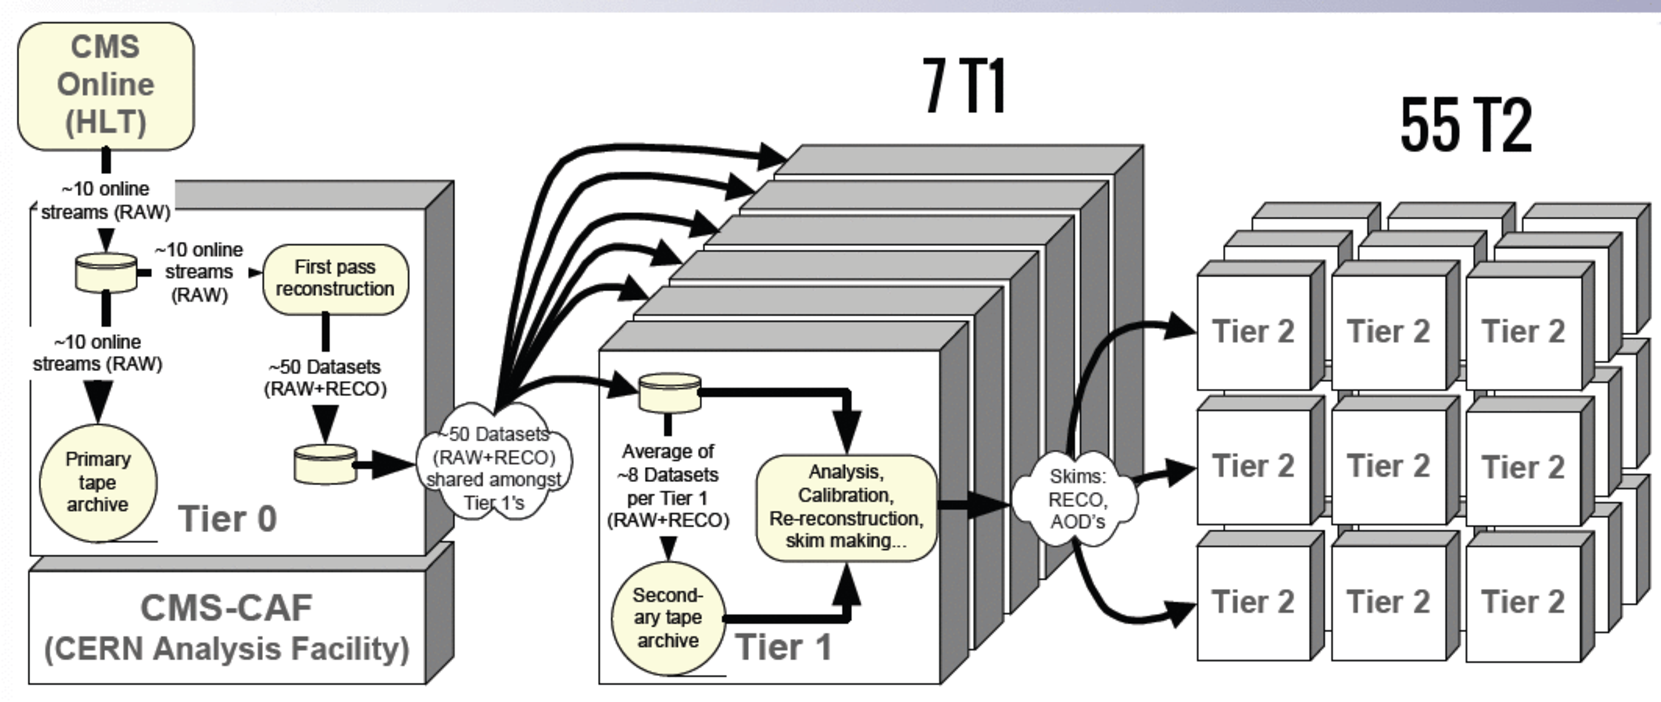
\includegraphics[width=0.90\linewidth]{Experiment/CMS/Image/data_tier_wf.pdf}
  \caption{The flow of collision data among different tiers. \cite{triDAS}}
  \label{fig:data_tier_wf}
  \end{center}
\end{figure}
